\documentclass[10pt]{article}

\usepackage[T1]{fontenc}
\usepackage[utf8]{inputenc}
\usepackage{lmodern}
\usepackage{amsmath}
\usepackage{amssymb}
\usepackage{pifont}
\usepackage{bm}
\usepackage{graphicx}
\usepackage[space]{grffile}
\usepackage{multicol}
\usepackage{array}
\usepackage{tabu}
\usepackage{ragged2e}
\usepackage{setspace}
\usepackage[font=small,labelfont=bf,labelsep=period]{caption}
%\usepackage{subcaption}
%\usepackage[CaptionAfterwards]{fltpage}
\usepackage{subfigure}
\usepackage{lineno}
\linenumbers
\usepackage{tikz}
\def\checkmark{\tikz\fill[scale=0.4](0,.35) -- (.25,0) -- (1,.7) -- (.25,.15) -- cycle;} 
\usepackage[margin=1.0in]{geometry}

\usepackage[backend=biber,style=authoryear,sorting=nyt,url=false,isbn=false,doi=false,firstinits=true]{biblatex}

\DeclareNameAlias{default}{last-first}

\DefineBibliographyStrings{english}{%
	andothers = {\addcomma\addspace\textsc{et\addabbrvspace al}\adddot},
	and = {\textsc{and}}
}
\renewcommand*{\labelnamepunct}{\space\space}

\renewbibmacro{in:}
{%
	\ifentrytype{article}{%
	}{%
		\printtext{\bibstring{in}\intitlepunct}%
	}%
}
\renewbibmacro*{volume+number}{%
	\printfield{volume}%
	\setunit*{\addcomma\space}%
	\printfield{number}%
	\setunit{\addcomma\space}}

\DeclareFieldFormat{pages}{#1}

\renewbibmacro*{publisher+location+date}{%
	\printlist{publisher}%
	\setunit*{\addcomma\space}%
	\setunit*{\addcomma\space}%
	\usebibmacro{date}%
	\newunit}

\renewcommand{\newunitpunct}{\addcomma\space}
\DeclareFieldFormat[article,inbook,incollection,inproceedings,patent,thesis,unpublished]{title}{#1} 
\DeclareFieldFormat{year}{#1} 

\renewcommand{\baselinestretch}{2.0}
\addbibresource{refs/ident_refs.bib}
\captionsetup{font={stretch=2.0}}

\begin{document}
	\begin{center}
		\begin{Large}
			Practical Identification and Experimental Design for Parameter Estimation in Kinetic Models of Metabolism
		\end{Large}\\
		Shyam Srinivasan\textsuperscript{a}, William R. Cluett\textsuperscript{a} and Radhakrishnan Mahadevan\textsuperscript{*,a,b}\\
	\end{center}
	a - Department of Chemical Engineering and Applied Chemistry, University of Toronto, Toronto, ON, Canada.\\
	b - Institute for Biomaterials and Biomedical Engineering, University of Toronto, Toronto, ON, Canada.\\
	{*} Corresponding author
	\section*{Abstract}
	\section{Introduction:}
	Kinetic models of metabolism can be used to study the dynamic characteristics of metabolic networks \parencite{Bordbar2015, Andreozzi2016}. 
	
	Unlike CBMs, where the ability to predict the steady state responses of metabolic networks is dependent on the stoichiometry of the network, the prediction of dynamic responses of metabolic networks to different perturbations using kinetic models of metabolism is also dependent on the numerical values of the enzyme kinetic parameters ($\theta$ in Equation \ref{eq:kinstoich}) \parencite{Andreozzi2016a}. Analyzing the ability of a metabolic network to exhibit dynamic characteristics like multiple steady states and oscillations, irrespective of the structure of the network, is one example where parameter values might play a crucial role \parencite{Srinivasan2015, Vital-Lopez2006}. The use of in vitro, or unreliable in vivo parameter estimates reduces confidence in the model predicted behaviour \parencite{Andreozzi2016a}. Consequently, the reduction in confidence hampers the use of these models to gain insight into the functioning of metabolic networks \parencite{Chakrabarti2013a, Bordbar2015}. The corresponding increase in uncertainty in model predicted responses becomes an obstacle for using the predicted responses as a basis for designing the metabolic networks to achieve any of the aforementioned goals of metabolic engineering and design.  
	
	Parameter estimation methods based on optimization principles are typically used to determine true parameter values based on available experimental data. Under the assumption that all time dependent intracellular metabolite concentrations can be measured, a parameter estimation problem can be formulated as a nonlinear programming problem (Equation \ref{eq:kinstoich}) to estimate the values of enzyme kinetic parameters, $\theta$, based on the measured data. 	
	The minimization of least square error between the measured ($x^*$) and modeled ($x$) concentrations, weighted by the variance in the experimental data $\sigma_{kl}^*$ for each concentration at each time point, is used as an objective function (Equation \ref{eq:lsqopt}a) for the optimization problem (Equation \ref{eq:lsqopt}). The parameter values are determined within fixed upper ($\theta_u$) and lower ($\theta_l$) bounds (Equation \ref{eq:lsqopt}b). 
	\begin{subequations}\label{eq:lsqopt}
		\begin{align}
		\underset{\theta}{\mathrm{min}} &\sum_{k=1}^{m}\sum_{l=1}^{d}\left(\frac{x_{kl}^*-x_{kl}}{\sigma_{kl}^*}\right)^2\\
		&\theta_l \le \theta \le \theta_u
		\end{align}
	\end{subequations}
	
	However, not all metabolite concentrations used in the model (Equation \ref{eq:kinstoich}) can be measured. Additionally, measurable fluxes in the metabolic network also need to be included as part of the parameter estimation problem. In such scenarios, the parameter estimation problem is modified to suit a new system of equations shown below (Equation \ref{eq:output}). The new system of equations is obtained by augmenting the original system (Equation \ref{eq:kinstoich}) with Equation (\ref{eq:output}c) that models the relationship between the measurable metabolite concentrations and fluxes ($y$) and the unmeasured concentrations ($x$) that are used in the original model (Equation \ref{eq:kinstoich}) above. The parameter vector ($\theta$) is augmented with additional parameters that define this relationship. These additional parameters also need to be estimated.
	\begin{subequations}\label{eq:output}
		\begin{align}
		\dot{x} = \mathbf{S}v\\
		v = f(x, y, \theta, u)\\
		\dot{y} = h(x, y, \theta, u)
		\end{align}
	\end{subequations}
	In systems identification, the measured concentrations and fluxes ($y$) are called output or observed variables, and the unmeasured concentrations ($x$) are called the state variables. For estimating $\theta$, the metabolite concentrations $x$ in the optimization problem (Equation \ref{eq:lsqopt}) are substituted with the output variables $y$. 
	
	The ability to determine unique solutions to parameters $\theta$ is governed by the identifiability of these parameters in the model \parencite{McLean2012, Raue2009a}. The identifiability of parameters in nonlinear models can be classified into two categories: structural (or a priori) and practical (or posterior) identifiability. 	
	Any system (Equation \ref{eq:output}) is said to be structurally identifiable if, for an input-output mapping defined by $y = \Phi(\theta,u)$ for at least one input function $u$, any two values of parameters $\theta_1$ and $\theta_2$ satisfy the relationship in Equation (\ref{eq:stident}) below.
	\begin{align}\label{eq:stident}
	\Phi(\theta_1,u) = \Phi(\theta_2,u) \iff \theta_1 = \theta_2
	\end{align}
	Accordingly, the system can have a unique solution, a finite number of non-unique solutions or an infinite number of solutions for all input functions, and is said to be structurally globally identifiable, locally identifiable or non-identifiable, respectively. So, the structural identifiability of parameters in a dynamic model helps establish the presence or absence of a relationship between the unobservable state variables and the observable output variables. Consequently, the effect of model structure and parameterization on the ability to infer true parameter values from experimental data is determined by the structural identifiability of the parameter. 
	
	Experimental data from many physical systems is usually noisy, and when parameters are estimated on the basis of noisy data, the ability to estimate unique parameter values to satisfy Equation (\ref{eq:stident}) is referred to as practical identifiability. So, the effect of the available experimental data on the ability to estimate unique parameter values is determined by the practical identifiability of the parameter. Accordingly, practical identifiability of a parameter is contingent upon the nature, quality and quantity of data available to estimate the parameter as opposed to the structure and parameterization of the model. 
	
	Thus, on the one hand, establishing the structural identifiability of parameters enables one to propose models that are not only appropriate representations of physical processes, but also are parameterized in such a way that the value of these parameters can be estimated from measurable data. On the other hand, establishing practical identifiability of parameters in any model helps design experiments that are minimal, informative and useful for parameter estimation.
	
	Methods and tools for structural identification of parameters based on differential algebra \parencite{Ljung1994, Audoly2001, Bellu2007} and profile likelihood \parencite{Raue2009a} are available. However, only the profile likelihood-based methods enable experimental design by facilitating practical identification of parameters. Nonetheless, this method still depend on solving a non-convex nonlinear least squares problem (Equation \ref{eq:lsqopt}) to get likelihood estimates of parameters, and hence still suffers from all the inherent difficulties associated with obtaining global optimal solutions for non-convex optimization problems. This also makes it un-scalable for experimental design and practical identifiability of parameters in kinetic models of large metabolic networks.
	
	In this paper, we propose a scalable methodology to establish practical identifiability for parameters in kinetic models of metabolism using steady state concentration and flux data. We present a computer algebra-based method that can facilitate experimental design through practical identification of parameters separately for each individual reaction within a metabolic network. For the purposes of this method we assume that all intracellular metabolite concentrations and fluxes can be measured. We identify and design experiments to estimate parameters in a small metabolic network model of glucoeneogenesis in \textit{Escherichia coli} \parencite{Kotte2014, Srinivasan2017} to illustrate the utility of our method.  %We also demonstrate the scalability of the proposed methodology to facilitate experimental design by applying it to a relatively larger metabolic network of the human red blood cell hepatocyte. 	
	
	\section{Methods}\label{sec:methods}
	\subsection{Kinetic models of metabolic networks}\label{sec:kinetic_model}
	In kinetic models of metabolism, ordinary differential equations (ode) are used to express the rate of change of metabolite concentrations ($x$) as a function of the reaction fluxes ($v$) in the metabolic network (Equation \ref{eq:kinstoich}). The matrix $\mathbf{S}$ in Equation (\ref{eq:kinstoich}a) defines the stoichiometric relationship between the fluxes and the concentrations of the metabolic network.
	\begin{subequations}\label{eq:kinstoich}
		\begin{align}
		\dot{x} = \mathbf{S}v\\
		v = f(x, \theta, u)
		\end{align}
	\end{subequations}
	The expression for the nonlinear function ($f$) used to describe each reaction flux $v_i$ in $v$, $i={1, 2, ..., n_r}$, in a kinetic model (Equation \ref{eq:kinstoich}b) is dependent on the enzyme kinetic mechanism that is used to model the reaction \parencite{Link2014, Srinivasan2015}. Accordingly, $f$ is a nonlinear function of the metabolite concentrations ($x$), enzyme kinetic parameters ($\theta$) and other input concentrations ($u$). 
	
	\subsection{A method to determine practical identifiability of kinetic models of metabolism}\label{sec:ident}
	We provide the mathematical framework for practical identification of parameters in kinetic models of metabolism in this section. A summary of the methodology in the form of a flow diagram is shown in Figure \ref{fig:ident-flowchart}. As indicated in Figure \ref{fig:ident-flowchart}a, the first step involves the construction of the kinetic model (Equation \ref{eq:kinstoich}) of the metabolic network with $n_r$ reaction fluxes.
	
	%In kinetic models of metabolic networks (Equation \ref{eq:kinstoich}), the fluxes are expressed as a function of the metabolite concentrations $x$ and the kinetic parameters $\theta$ (Figure \ref{fig:ident-flowchart}a). The value of every flux $v_i$, $i={1, 2, ..., n_r}$, is expressed using one of the many available enzyme kinetic formulations (Equation \ref{eq:output}b). Without loss of generality, all of these kinetic formulations can be expressed as nonlinear algebraic equations (Figure \ref{fig:ident-flowchart}a). 	
	
	For each flux $v_i$, $i={1, 2, ..., n_r}$, in the kinetic model, let $\mathbf{\theta} \in \mathbb{R}^p$ in Equation (\ref{eq:kinstoich}b). If data from $n_E$ experiments is available for the chosen metabolic network, as stated earlier, for each experiment $j = {1, 2, ..., n_E}$, we assume that all metabolite concentrations ($x$) and reaction fluxes ($v$) are measurable. We discuss the implications of relaxing this assumption later. The pertinent information for each experiment $j$ is available as a vector of concentrations and fluxes, $\mathbf{x}_j$ and $\mathbf{v}_j$, respectively (Figure \ref{fig:ident-flowchart}b). 
	
	In order to establish the practical identifiability of kinetic parameters for each flux $v_i$, $i={1, 2, ..., n_r}$, we describe a computer algebra-based method. The primary use of the computer algebra system is to obtain closed-form expressions for each parameter in $\mathbf{\theta}$ for each flux $v_i$ (Figure \ref{fig:ident-flowchart}b). This is done by first selecting a combination of $p$ data sets from the $n_{E}$ available experimental data sets. The combination consisting of data from $p$ different experiments is then used to formulate a system of nonlinear algebraic equations in $\mathbb{R}^p$ for each flux $v_i$, shown in Equation (\ref{eq:nonlineq}). 
	\begin{align}\label{eq:nonlineq}
	v_{i, j} = f_j(\mathbf{x}_j,\mathbf{\theta}, \mathbf{u}_j) && \forall j=\{1, 2, ..., p\}\subset\{1, 2, ..., n_E\}
	\end{align}
	Here, $v_{i,j}$ refers to the value of the flux $v_i$ obtained from experiment $j$, $\mathbf{x}_j$ and $\mathbf{u}_j$ are the vector of metabolite and other input concentrations from each experiment $j$, and $\mathbf{\theta}$ is a vector in $\mathbb{R}^p$.
	
	Each equation in (\ref{eq:nonlineq}), indicated by the index $j$, corresponds to the kinetic rate law expression $f(x, \theta, u)$ for each $v_i$, $i={1, 2, ..., n_r}$, described in Equation (\ref{eq:kinstoich}b), written for concentrations ($\mathbf{x}_j$, $\mathbf{u}_j$) and fluxes ($v_{i,j}$) obtained from experiment $j$. Solving the system in Equation (\ref{eq:nonlineq}) results in $\mathbb{R}^p$ nonlinear expressions for parameters in $\theta$ (Equation \ref{eq:theta-eq}), where $N(\mathbf{v}_i, \mathbf{x}, \mathbf{u})$ is the numerator of $g$, and $D(\mathbf{v}_i, \mathbf{x}, \mathbf{u})$ is the denominator of $g$ (Figure \ref{fig:ident-flowchart}b). Note that $\mathbf{v}_i$, $\mathbf{x}$ and $\mathbf{u}$ are used to denote vector of vectors of fluxes for reaction $i$ ($\mathbf{v}_i$), metabolite ($\mathbf{x}$) and input ($\mathbf{u}$) concentrations, respectively, obtained from all chosen experiments $j = {1, 2, ..., p}$, in the selected combination.
	\begin{align}\label{eq:theta-eq}
	\theta_j = g_j(\mathbf{v}_i, \mathbf{x}, \mathbf{u}) = \frac{N_j(\mathbf{v}_i, \mathbf{x}, \mathbf{u})}{D_j(\mathbf{v}_i, \mathbf{x}, \mathbf{u})}
	\end{align}
	The identifiability of parameter $\theta_j$, $j = {1, 2, ..., p}$, for flux $v_i$ can be established by determining the value of $D_j(\mathbf{v}_i, \mathbf{x}, \mathbf{u})$ (Figure \ref{fig:ident-flowchart}b): any parameter $\theta_j$ is said to practically identifiable if $D_j(\mathbf{v}_i, \mathbf{x}, \mathbf{u})\neq0$, and practically non-identifiable if $D_j(\mathbf{v}_i, \mathbf{x}, \mathbf{u}) = 0$. Furthermore, the physical properties of the kinetic parameters can be used to distinguish between identifiable and non-identifiable parameter values by designating only parameters with a non-negative value of $g_j(\mathbf{v}_i, \mathbf{x}, \mathbf{u})$ as identifiable (Figure \ref{fig:ident-flowchart}b). The solution obtained for $g_j(\mathbf{v}_i, \mathbf{x}, \mathbf{u})$ in Equation (\ref{eq:theta-eq}) is unique for an identifiable $\theta_j$, and an infinite number of solutions are possible for a non-identifiable $\theta_j$. However, if there are multiple but finite solutions for $g_j(\mathbf{v}_i, \mathbf{x}, \mathbf{u})$, then the corresponding parameter $\theta_j$ is locally identifiable.
	
	%For completeness, in the following sections we provide a previously published kinetic model of a small gluconeogenic network (section \ref{sec:small-model}). 
	
	\subsection{Degree of identifiability: A quantitative measure of practical identifiability}\label{sec:degree_of_identifiability}
	We express the practical identifiability of kinetic parameters using a simple quantitative term called the degree of identifiability. We describe the degree of identifiability of any single parameter as the percentage of all data combinations (used to test for practical identifiability) that can identify that parameter. 
	
	As an example, if 90\% of all the experimental data combinations used for testing can identify a parameter $\theta_i$, then the degree of identifiability of $\theta_i$ is said to be 0.9 or 90\%. On the other hand, if only 50\% of the combinations can identify another parameter $\theta_j$, then $\theta_j$ has a degree of identifiability of 0.5 or 50\%. Furthermore, we can create a hierarchy of practically identifiable parameters using their degrees of identifiability. In the above instance of the two parameters $\theta_i$ and $\theta_j$ that have degrees of identifiability of 90\% and 50\% respectively, $\theta_i$ is classified to be more identifiable than $\theta_j$ due to its relatively higher degree of identifiability. 
	
	Determining this hierarchy of identifiable parameters can help in distinguishing parameters that can be identified by any type and any combination of experiments from parameters that can be identified by only a select type and combination of experiments. Such a classification can subsequently be used to design minimal sets of experiments that can practically identify all kinetic parameters used to model a metabolic network, going from the least identifiable parameter to the most identifiable parameter.  
	
	\subsection{Kinetic model of gluconeogenesis in \textit{E. coli}}\label{sec:small-model}
	A previously proposed kinetic model \parencite{Kotte2014, Srinivasan2017} for acetate consumption through gluconeogenesis (Figure \ref{fig:network}) is used as a case study to illustrate the utility of identifiability analysis for experimental design for parameter estimation in kinetic models of metabolism. The kinetic model is described below.
	
	\begin{equation}\label{eq:ode1}
	\frac{d}{dt}pep=v_1-v_2-v_4
	\end{equation}
	\begin{equation}\label{eq:ode2}
	\frac{d}{dt}fdp=v_2-v_3
	\end{equation}
	\begin{equation}\label{eq:ode3}
	\frac{d}{dt}E=v_{e,max}\left(\frac{1}{1+\left(\frac{fdp}{K_{e}^{fdp}}\right)^{n_e}}\right) - d E
	\end{equation}
	The kinetic expressions for fluxes $v_1$ through $v_4$ are given below. The consumption of acetate through $v_1$ and conversion of \textit{pep} through $v_2$ are expressed in Equations (\ref{eq:flux1}) and (\ref{eq:flux2}) respectively using Michaelis-Menten kinetics. The acetate flux through $v_1$ is also governed by the quantity of available enzyme E. 
	\begin{equation}\label{eq:flux1}
	v_1 = k_{1}^{cat}E\frac{ac}{ac+K_{1}^{ac}}
	\end{equation}	
	\begin{equation}\label{eq:flux2}
	v_2 = V_{2}^{max}\frac{pep}{pep+K_{2}^{pep}}
	\end{equation}
	\begin{equation}\label{eq:flux3}
	v_3 = V_{3}^{max}\frac{\tilde{fdp}\left(1+\tilde{fdp}\right)^3}{\left(1+\tilde{fdp}\right)^4+L_3\left(1+\frac{pep}{K_{3}^{pep}}\right)^{-4}}
	\end{equation}
	The allosterically regulated flux $v_3$ for the consumption of \textit{fdp} is expressed in Equation (\ref{eq:flux3}) using the Monod-Wyman-Changeux (MWC) model for allosterically regulated enzymes, where $\tilde{fdp}$ refers to the ratio of \textit{fdp} with respect to its allosteric binding constant $K_{3}^{fdp}$. The flux $v_4$ for the export of \textit{pep} is expressed as a linear equation dependent on $pep$ in Equation (\ref{eq:flux4}).
	\begin{equation}\label{eq:flux4}
	v_4 = k_{4}^{cat}.pep
	\end{equation}	
	
	\subsection{Data for establishing parameter identifiability in kinetic model of gluconeogenesis}\label{sec:experiments}
	Steady state information on the metabolome and the fluxome can be gathered under different physiological conditions. One way to alter the physiological conditions is to change the substrate concentration under which the cells grow. In the small metabolic network (Figure \ref{fig:network}), the acetate concentration plays the role of a substrate, and  determines the acetate uptake flux $v_1$. Thus, steady state metabolite concentrations and fluxes can be calculated under various acetate concentrations to form different experimental data combinations that measure cellular response to changes in the substrate concentration. 
	
	Physiological changes can also be brought about by perturbing the expression levels for different enzymes within a metabolic network. The model of gluconeogenesis (Figure \ref{fig:network}) described in section \ref{sec:small-model} has three different fluxes ($v_1$, $v_2$ and $v_3$) whose enzyme expression parameters ($k_1^{cat}$, $V_2^{max}$ and $V_3^{max}$) can be perturbed to simulate the repression and over expression of the corresponding enzymes. Accordingly, in addition to measuring network response to substrate perturbations, changes in steady state concentrations and fluxes can also be observed for enzyme expression perturbations.
	
	In total, based on the above discussion, we can perturb four different model parameters ($acetate$, $k_1^{cat}$, $V_2^{max}$ and $V_3^{max}$) to obtain experimental data in silico. The 21 different parameter values used to generate experimental data are given in Table \ref{tab:pval}.	
	
	As described previously in section \ref{sec:ident} and Figure \ref{fig:ident-flowchart}b, the minimum number of experiments from which steady state data is required for identifying all the parameters of a given flux is determined by dimension $\mathbb{R}^p$ of the parameter space of a chosen flux $v_i$. For instance, the flux $v_2$ in the model described in section \ref{sec:small-model} has two parameters: $V_2^{max}$ and $K_2^{pep}$. Thus $\theta = \{V_2^{max}, K_2^{pep}\} \in \mathbb{R}^2$. So, steady state data from two distinct experiments is required for identifying $v_2$. Accordingly, multiple combinations of data generated from any two different experiments are used to test the identifiability of $v_2$. The total number of such possible combinations is 420 (21 x 20) from the 21 different experiments shown in Table \ref{tab:pval}. Assuming we also have data for the enzyme concentration $E$ in the expression for flux $v_1$ (Equation \ref{eq:flux1}), identifying the two parameters $k_1^{cat}$ and $K_1^{ac}$ ($\theta \in \mathbb{R}^2$) also requires steady state experimental data from two different experiments.
	
	Similarly, for identifying $v_3$ that is described by three parameters ($\theta \in \mathbb{R}^3$), we need data from a combination of three different experiments. Based on the 21 experiments in Table \ref{tab:pval}, we have 7980 distinct combinations (21 x 20 x 19) of three experiments. However, it is important to note that not all of the either 420 combinations (for $v_1$ and $v_2$), or the 7980 combinations (for $v_3$), may be suitable for parameter estimation. Hence, the actual number of data combinations that can be used for practically identifying parameters in these fluxes would be smaller than the aforementioned numbers. Moreover, among these chosen smaller number of experimental data combinations, our methodology enables us to calculate the number of experimental data combinations, and consequently, the number of experiments that might allow for parameter identification, and subsequent parameter estimation. The following section describes a procedure that can be used to design experiments within this context.	
	
	\subsection{Experimental design through practical parameter identification}\label{sec:experimental_design}	
	Following the methodology described in section \ref{sec:ident}, and demonstrated in section \ref{sec:example} for a single flux using data from a combination of two different experiments, all distinct combinations found based on experiments described in section \ref{sec:experiments} can be tested for their ability to practically identify any of the three fluxes in the small metabolic network. This step would determine the degree of identifiability (defined in section \ref{sec:degree_of_identifiability}) of each parameter in each flux in the model, and help distinguishing experiment combinations that contribute to identifiability from combinations that do not practically identify any parameter in the model (Figure \ref{fig:ident-flowchart}b). In doing so, it is possible to obtain a minimal and informative collection of experiments that can be performed to identify as many model parameters as possible (Figure \ref{fig:ident-design}). Consequently, the set of experiments can be used to estimate the identifiable parameters in the model. This is formally explained below.
	
	The identifiability of each parameter based on each experiment indexed as $j = \{1, ..., n\}$ is established based on the methodology described previously in section \ref{sec:ident} and demonstrated in Section \ref{sec:example} (Figure \ref{fig:ident-flowchart}b). Subsequently, for any flux $v_i$ and for any $p$ combinations of indices $j$, if the experimental concentrations ($\mathbf{x}_j$) and fluxes ($\mathbf{v}_j$) do not satisfy the condition for identifiability for any parameter $\theta_k$ in $\theta\in\mathbb{R}^p$, i.e., $D_k(\mathbf{v}_i, \mathbf{x}, \mathbf{u}) = 0$ for any $k$, then at least one of the $p$ experiments needs to be changed to make parameter $\theta_k$ identifiable. Consequently, the corresponding experiment cannot be used for parameter estimation and needs to be discarded from the set of all necessary experiments. Furthermore, another experiment from $j = \{1, ..., n\}$ needs to be selected such that parameter $\theta_k$ is identifiable. This process has to be repeated until all parameters in $\theta\in\mathbb{R}^p$ are identifiable for flux $v_i$. In doing so, we can arrive at a set of $p$ experiments that will always result in practically identifiable parameters for flux $v_i$. Note that if none of the $n$ pre-selected experiments satisfy the identifiability condition, then we can design an $(n+1)^{th}$ experiment that can replace one of the experiments that causes practical non-identifiability. This analysis can be performed for each flux in a metabolic network independent of all the other fluxes, making it theoretically scalable even to genome-scale models of metabolism. 	
	
	\section{Results:}
	First in section \ref{sec:closedform}, we show that the ability to establish practical identifiability of kinetic parameters in metabolic network models using our methodology, described in section \ref{sec:ident}, relies upon the nonlinearity of the kinetic rate law formulations used to describe the fluxes. We use the gluconeogenic model (Figure \ref{fig:network}) described in section \ref{sec:example} as an example. 
	
	%In the following section we demonstrate our methodology to establish practical identifiability for one of the fluxes in this network (section \ref{sec:example}) (move to results).
	
	Then, in section \ref{sec:data_utility} we provide a motivation for the need for experimental design, especially to identify kinetic models of metabolic networks. We do this by looking at the number of combinations that can identify the maximum number of parameters. 
	In section \ref{sec:trends} we show that the degree of identifiability of the maximum reaction rate parameter is always higher than the degree of identifiability of the corresponding enzyme binding parameter irrespective of enzyme kinetic rate law used to describe the flux. 
	In section \ref{sec:experiment_type} we discuss the ability to determine the type of experiments for parameter identification for a given flux based on the informativeness of a given type of experiment. In this section we show how the informativeness of a given type of experiment to identify a specific flux can be deduced from its contribution towards the practical identification of the parameters for a given flux. Finally, we discuss some results arising out of the use of our methodology to determine the identifiability of parameters when data with additive noise is used in section \ref{sec:noise}.
	
	\subsection{Identifiability of parameters in a kinetic model of gluconeogenesis}\label{sec:example}
	Here, we demonstrate the use of our computer algebra-based methodology to establish practical identifiability of parameters for flux $v_1$ in the small model of gluconeogenesis (Figure \ref{fig:network}) described in section \ref{sec:small-model}. 
	
	In flux $v_1$, the concentration of the enzyme E is used as a variable. Since we assume that steady state experimental information is only available for metabolite concentrations and fluxes, the expression previously given for $v_1$ (Equation \ref{eq:flux1}) cannot be used for identifying parameters $k_1^{cat}$ and $K_1^{ac}$. So, we modify the Michaelis-Menten kinetic rate law expression to eliminate the enzyme concentration E as a variable in Equation (\ref{eq:flux1a}). Consequently $k_1^{cat}$ is replaced by $V_1^{max}$ as a parameter to describe $v_1$. The corresponding enzyme binding constant is denoted as $K_1^{ac} (ne)$ to distinguish it from the enzyme binding constant calculated in the presence of measured enzyme concentration data.
	\begin{align}\label{eq:flux1a}
	v_1 = V_1^{max}\frac{ac}{ac+K_{1}^{ac}(ne)}
	\end{align}		
	We choose the expression for flux $v_1$ given in Equation (\ref{eq:flux1a}) to demonstrate our method for practical identifiability. 
	
	As mentioned in section \ref{sec:intro}, practical identifiability is a necessary condition to estimate true values of both $V_1^{max}$ and $K_1^{ac}$ from experimental data. Here, we assume that the concentrations and fluxes from at least two different experiments are available i.e., in Equation (\ref{eq:nonlineq}) $k = \{1, 2\}$ . We label the available concentrations and fluxes as ${ac}^{(k)}$ and ${v_1}^{(k)}$, respectively. Then, the nonlinear algebraic equations shown in Equation (\ref{eq:nonlineq}) can be formulated for $v_1$ as:
	\begin{align}\label{eq:nonlin-flux2}
	{v_1}^{(k)} = V_{1}^{max}\frac{ac^{(k)}}{ac^{(k)}+K_{1}^{ac}(ne)} &&  k=\{1, 2\}
	\end{align}
	
	Solving this simultaneous system of $k$ equations using Mathematica (Wolfram Research, USA), a computer algebra system, we get $p=2$ nonlinear algebraic expressions for parameters $V_1^{max}$ (Equation \ref{eq:v1_par}a) and $K_1^{ac}(ne)$ (Equation \ref{eq:v1_par}b). These expressions have the form previously shown in Equation (\ref{eq:theta-eq}).
	\begin{subequations}\label{eq:v1_par}
		\begin{align}		
		V_1^{max} = \frac{v_1^{(1)}v_1^{(2)}(ac^{(1)}-ac^{(2)})}{v_1^{(2)}ac^{(1)}-v_1^{(1)}ac^{(2)}}\\
		K_1^{ac}(ne) = \frac{ac^{(1)}ac^{(2)}(v_1^{(1)}-v_1^{(2)})}{v_1^{(2)}ac^{(1)}-v_1^{(1)}ac^{(2)}}
		\end{align}
	\end{subequations}
	In Equation (\ref{eq:v1_par}), the denominator of the right hand side expression is used to test the identifiability of parameters $V_1^{max}$ (Equation \ref{eq:v1_par}a) and $K_1^{ac}(ne)$ (Equation \ref{eq:v1_par}b) for different available experimental data combinations. Since the enzyme binding constant ($K_1^{ac}(ne)$) and the maximum reaction rate ($V_1^{max}$) cannot be negative, we can further constrain the criteria for identifiability for both these parameters by saying that the evaluated expressions in Equation (\ref{eq:v1_par}) should be non-negative (Figure \ref{fig:ident-flowchart}b). 	
	
	\subsection{Nonlinearity of enzyme kinetic rate law expression affects identifiability analysis}\label{sec:closedform}
	Practical identifiability of parameters in kinetic models of metabolism using the methodology described in section \ref{sec:methods} is governed by the nonlinear complexity of the enzyme kinetic rate law used to model a specific flux. We demonstrate one example of how the methodology works in section \ref{sec:example} for parameters of flux $v_1$. The expression in Equation (\ref{eq:v1_par}) is obtained by using a computer algebra system. To recall, in this specific case, a computer algebra system is used to solve for the parameters of a flux described using the Michaelis-Menten kinetic rate law when data from two different experiments is available. 
	
	However, we find that the nonlinearity of the MWC kinetic rate law used to model the allosteric regulation of $v_3$ makes it computationally intractable for determining the closed form expressions of the three parameters $V_3^{max}$, $K_3^{fdp}$ and $K_3^{pep}$ using a computer algebra system (Mathematica and SymPy in Python). In order to overcome this computational obstacle, we model the reaction rate for $v_3$ using the convenience kinetic rate law formulation \parencite{Liebermeister2006}. The corresponding expression obtained for $v_3$ is given below (Equation \ref{eq:flux3_convkin}). 
	
	\begin{align}\label{eq:flux3_convkin}
	v_3 = V_3^{max}\left(\frac{1}{1 + \frac{K_3^{pep}}{pep}}\right)\left(\frac{\frac{fdp}{K_3^{fdp}}}{1 + \frac{fdp}{K_3^{fdp}}}\right)
	\end{align}
	
	Using this expression for analysis, we find that each of the parameters $V_3^{max}$, $K_3^{fdp}$ and $K_3^{pep}$ have two different closed-form expressions owing to the presence of a square root term in their solutions. These distinct expressions are denoted by (1) and (2) following the respective parameter names throughout the rest of the document: $V_3^{max}(1)$, $K_3^{fdp}(1)$, $K_3^{pep}(1)$, and $V_3^{max}(2)$, $K_3^{fdp}(2)$, $K_3^{pep}(2)$. 
	
	The impact of nonlinearity of a kinetic rate law expression affecting the practical identifiability of parameters in the expression may not be an unique problem isolated to the system that we are investigating. Complicated expressions for describing fluxes have been extensively used to model observed experimental data for different fluxes in a variety of organisms \parencite{Chassagnole2002a, Peskov2012, VanHeerden2014}. However, the identifiability of the parameters used in these models has never been truly examined. Unlike the case of the MWC model, if determining closed-form expressions for the parameters of these models are tractable, we believe our methodology can help in elucidating the identifiability of these parameters. If not, metabolic network fluxes can be expressed using alternative kinetic rate law models whose parameters can be tested for identifiability, and subsequently experiments can be designed for their estimation and model validation.
	
	Next, we look at some of the results we obtained for the practical identification of different parameters for all three fluxes $v_1$, $v_2$ and $v_3$ in the small gluconeogenic network model described in section \ref{sec:small-model}, with the flux for $v_3$ described by Equation (\ref{eq:flux3_convkin}). We start by looking at one of motivations for the need for designing experiments to collect data for parameter estimation.
	
	
	\subsection{Utility of experimental data for practical parameter identification}\label{sec:data_utility}
	Although the need for better parameter estimation methods is well researched, within the kinetic modeling community, the need for experimental design methods to satisfy the data needs for parameter estimation are not considered seriously. Hence, we find the need to stress the necessity for experimental design methodologies, in this case, tailored specifically for metabolic network models. 	
	
	We do this by showing how useful the multiple combinations of experimental data are towards identifying parameters for each given flux (Figure \ref{fig:figure4}). We express the usefulness of any given data combination on the basis of the number of parameters that the combination can identify. The higher the number of parameters a data combination can identify, the greater is the usefulness of that combination of experiments. 
	
	The number of data combinations that can identify a specific number of parameters within a given flux is shown in Figure \ref{fig:figure4}. The percentage of all data combinations that can estimate a given number of parameters within a given flux are also shown in Figure \ref{fig:figure4}. For flux $v_1$ (Figure \ref{fig:figure4}a) about 78\% of the 306 data combinations cannot identify any parameter used to model the flux ($V_1^{max}$ and $K_1^{ac}(ne)$). Only a single parameter can be identified by about 2\% of the combinations, while only about 19\% of the data combinations can identify both the parameters used in the model. 	
	In contrast, most data combinations (>90\%) are not wasted, and can identify both parameters in $v_2$ (Figure \ref{fig:figure4}b). Less than 5\% of the experimental data combinations are wasted from not being able to identify any parameter. In the case of $v_3$ (Figure \ref{fig:figure4}c), about 45\% of the 4896 data combinations can identify only one parameter, while 13\% of the combinations cannot identify any parameter. Only 10\% of combinations can identify $v_3$ completely. 
	
	Thus, Figure \ref{fig:figure4} gives credence to the idea that careful experimental design is necessary to minimize usage of resources devoted to performing experiments for parameter estimation. For instance, choosing any of the experiment combinations from the 78\% percent that does not identify any parameter in $v_1$, or the 13\% that does not identify any parameter in $v_3$ can lead to experiments that are not informative. This can lead to potential waste of resources used to perform these experiments.	 
	
	In addition to providing information on the fraction of experiments that are informative and those that are not informative, Figure \ref{fig:figure4} also informs on the ease of identifying parameters for a single flux. For the small network (Figure \ref{fig:network}), we find that more than 90\% of all the data combinations tested for their ability to identify $v_2$ are actually capable of identifying $V_2^{max}$ and $K_2^{pep}$ (Figure \ref{fig:figure4}b). In contrast, less than 20\% of the combinations can identify both parameters in $v_1$. Since minimization of resource utilization requires us to use the least number of experiments to identify both $v_1$ as well as $v_2$, this indicates the need to carefully choose combinations of experiments that can identify $v_1$. A careful consideration of experiments for identifying $v_2$ is however not a major concern since there is a very high probability that experiments chosen to identify $v_1$ will also identify $v_2$. 	
	
	Although the calculation of the utility of experiment combinations in terms of their ability to identify the maximum number of parameters gives an idea on the informativeness of experiments used to gather the data, further analysis from the perspective of identifiability of the parameters of different fluxes is required to be able to design experiments based on this information. Hence, we look at the degree of identifiability (see section \ref{sec:degree_of_identifiability}) of each parameter of each flux in the following section to be able to classify parameters, and consequently fluxes, from most identifiable to least identifiable.
	
	\subsection{Maximum reaction rates are more identifiable than enzyme binding constants}\label{sec:trends}	
	In Figure \ref{fig:figure1} we show the number and percentage of combinations that are capable of identifying each parameter in each flux. Based on the definition given in section \ref{sec:degree_of_identifiability}, the percentages refer to the degree of identifiability of each parameter. The three panels in Figure \ref{fig:figure1} represent the degree of identifiability for parameters modeling the three different fluxes of the small network individually. 
	
	In regards to the identifiability of $v_1$ (Figure \ref{fig:figure1}a), $v_2$ (Figure \ref{fig:figure1}b) and $v_3$ (Figure \ref{fig:figure1}c), the degree of identifiability of the maximum reaction rates ($V_i^{max}$) in each of the three fluxes is higher than the degree of identifiability of the corresponding enzyme binding ($K_i$) constants and the allosteric activation constant ($K_3^{pep}$). We observe this trend irrespective of the fact that only  $v_1$ and $v_2$ are represented by the same enzyme kinetic rate law (Michaelis-Menten), while the convenience kinetic rate law is used to model $v_3$. These observations lead us to conclude that the maximum reaction rate parameters are always more identifiable (as indicated by their higher degree of identifiability) than their enzyme binding constant counterparts, irrespective of the enzyme kinetic rate law used to model the corresponding flux.
	
	From Figure \ref{fig:figure1} we see that the variation in the degree of identifiability is not only dependent on the type of parameter being identified, but is also associated with the flux that these parameters model.	In systems identification terminology, this can be tied to selecting experiments that are persistently excitable for the flux being identified. In systems identification, any input signal should be rich or informative enough to guarantee full excitement of the dynamics of the system \parencite{Ljung1994}. Only information obtained from such changes in the input can be used to completely identify the system over its entire dynamic range. Input signals that guarantee to fully excite the dynamics of the system are termed as persistently excitable signals. In linear systems, persistence of excitation of any input signal can be theoretically guaranteed. However, for nonlinear systems, like the metabolic network we deal with in this paper, persistence of excitation of input signals cannot be theoretically guaranteed, and should be assessed on a case by case basis. The lack of persistence of excitation requires the design of experiments to satisfy the data needs for complete system identification. 
	
	In the case of identifying fluxes within a metabolic network individually, each flux is not independent from the other fluxes that form the metabolic network. Each flux is connected to one or more fluxes through the metabolites that not only act as substrates and products, but also as allosteric activators and inhibitors (e.g., effect of \textit{pep} on $v_3$ in Figure \ref{fig:network}). Hence, careful consideration of experiments is a necessity so that the data acquired can satisfy conditions for practical identifiability for all parameters modeling a flux, and subsequently, all fluxes within a network. In the next section we discuss the dependence of the variation in the degree of identifiability for parameters of different fluxes from the point of view of the informativeness of experiments from which data is collected for identification.
	
	\subsection{Experiment requirements for identifying parameters depend on the position of the flux in the metabolic network}\label{sec:experiment_type}	
	In this section, we demonstrate a specific case of lack of persistence of excitation and the subsequent experimental design required to overcome this hurdle for parameter identifiability for a small nonlinear metabolic network model. Earlier, we mentioned that the informativeness of experiments for identifying parameters in a given flux depends on its ability to satisfy the conditions determined for practical identifiability of that parameter. For example, we demonstrated in section \ref{sec:example} that for a combination of any two experiments to be capable of identifying $V_1^{max}$ and $K_1^{ac}$ in $v_1$, the experiments must have distinct acetate concentrations as well as a different uptake flux $v_1$ between them (Equation \ref{eq:v1_par}). Thus, in this instance, the informativeness of the experiments (changes in the input acetate concentration and $v_1$) for identifying parameters of $v_1$ is determined by the ability of the input change to effect a change in the measured value of $v_1$. Similarly, the identification of parameters for $v_2$ requires the experiments to distinguish between values of both $v_2$ as well as \textit{pep}. %, given both these variables are outputs of the model describing $v_2$. 
	
	As such, as per Figure \ref{fig:figure1}a only 20\% of all data combinations can satisfy these requirements, and can consequently identify $v_1$. Whereas, more than 90\% of the available data combinations satisfy the requirements for identifying $v_2$ (Figure \ref{fig:figure1}b). Thus, identifiability analysis is crucial to determine the minimum number of experiments, as well as the nature of experiments that can help identify parameters for both $v_1$ and $v_2$. Recall that we use experimental data from five different types of experiments to test the practical identifiability of parameters in the model (Section \ref{sec:experiments}).
	In order to determine the type of experiments that help satisfy identifiability conditions for both parameters of $v_1$, we look at the distribution of the five different types in all data combinations that can identify these 2 parameters (Figure \ref{fig:figure2}a and b).	
	
	The contribution of experiments that involve changes in the acetate concentrations, which consequently bring about changes in the value of $v_1$, contribute to a significant part (> 50\%) of the identifiable experimental data combinations in comparison to the other types of experiments. This matches with requirements for identifiability on the basis of the informativeness of experiments that was laid out earlier i.e., experiments must be able distinguish between different values of $v_1$ and acetate. Accordingly, only about 20\% of the 306 different experiment combinations used to test identifiability are informative enough to discriminate both acetate as well as $v_1$, and can identify $V_1^{max}$ and $K_1^{ac}(ne)$ (Figure \ref{fig:figure1}a). 	
	
	In contrast to $v_1$, we see that the different enzyme perturbation experiments have a higher contribution towards data combinations that can identify parameters for $v_2$ (Figure \ref{fig:figure2}c and d). Hence, in conjunction with the high degree of identifiability seen in Figure \ref{fig:figure1}b for $v_2$, we can deduce that almost all experiment types are persistently excitable for $v_2$ i.e., most experiments can bring about noticeable changes to both \textit{pep} and $v_2$. Consequently, in comparison to selecting experiments to identify $v_1$, there is very little restriction on the types of experiments that are informative enough to identify $v_2$. This observations is in line with the one made in section \ref{sec:data_utility} based on the total number of combinations that can identify both parameters in $v_2$.
	
	Both the degree of identifiability of parameters and the informativeness of the corresponding experiments used to identify them can be explained by the position of the flux in the metabolic network. The position of any given flux in the metabolic network determines the specific experiment that is persistently excitable enough to identify the parameters of that flux. This dependency of experiment informativeness on the position of the flux can be further elucidated using $v_1$ and $v_2$ as examples. We know from Equation (\ref{eq:v1_par}) that identifiability of $v_1$ requires changes in both acetate and $v_1$. We also know, based on our knowledge of the Michaelis-Menten kinetic rate law that changes in the substrate concentration of a reaction can bring about a nonlinear change in the value of the corresponding reaction rate. In this specific metabolic network, since the substrate is an input variable to the model, and $v_1$ is the corresponding uptake flux, the substrate can be easily perturbed to create persistently excitable experiments to identify parameters in $v_1$. We can generalize this observation for the identification of all uptake fluxes in all metabolic networks, i.e., at a minimum, a change in the input substrate concentration may be necessary for an informative experiment to identify the uptake flux parameters. 
	
	On the other hand, the Michaelis-Menten model for $v_2$ also requires changes in \textit{pep} and $v_2$ for persistently excitable experiments to identify $v_2$. However, since both of these are system outputs, satisfaction of this condition cannot be guaranteed without an analysis of the dynamics of the metabolic network and how changes in the input (acetate) bring about changes in the two requisite output quantities. Previous dynamical analysis of the network (Figure \ref{fig:network} in the Appendix) has already established the existence of a functional relationship between \textit{pep} and $v_2$, and the input acetate concentration and the levels of expression of the different enzymes within the network \parencite{Srinivasan2017}. Hence, it is theoretically possible for any of the five different experiment types to be persistently excitable to identify $v_2$. This is confirmed by the high degree of identifiability for both parameters of $v_2$, where in more than 90\% of all data combinations can identify the parameters. Thus, this analysis informs us that the degree of identifiability and consequently, the type of experiments needed to identify different parameters varies widely depending on the position of the flux in the metabolic network with respect to the inputs and the outputs of the network, as well as the various regulatory interactions present within the network. We can extend these observations to justify the observed contribution of experiments towards identifying parameters for $v_3$ as well (Figure \ref{fig:figure2_v3}).	
	
	\subsection{Effect of noise on degree of identifiability is dependent on nonlinearity of enzyme kinetic rate law models}\label{sec:noise}
	In reality, experimental data from biological systems is usually noisy. Noise in data gathered from experiments is associated with biological noise attributable to the stochasticity of cellular function, as well as measurement noise associated with the techniques used to obtain concentration and flux measurements. However, the previous sections describe practical identifiability for parameters obtained using noise-free in silico experimental data. So, in order to illustrate the ability of our method to test the practical identifiability of parameters under realistic circumstances, we apply our methodology on in silico data (concentration and flux) with 5\% additive noise. 
	
	50 different samples of noise with 0 mean and 5\% standard deviation are drawn from a normal distribution and added to the steady state experimental data generated on the basis of experiments described in Section \ref{sec:experiments} to generate 50 different samples of noisy data. Subsequently, all 50 samples are tested for their ability to practically identify all three fluxes of the small network (Figure \ref{fig:network}). The degree of identifiability of the different parameters using noisy experimental data are shown in the Appendix (Figure \ref{fig:figure1_noisy}). 
	
	We hypothesize that the nonlinearity of the enzyme kinetic rate law used to model a flux, and consequently the complexity of the closed form expression obtained for the various parameters used in the model has an impact on the ability of noisy data to practically identify the parameters. The difference in the identifiability attributable to the aforementioned factors can be seen in the difference in the degree of identifiability for the parameters of $v_1$, $v_2$ and $v_3$ in the small metabolic network that we use to demonstrate our methodology. 
	
	Despite the presence of noise, the degree of identifiability of $v_1$ and $v_2$ (Figure \ref{fig:figure1_noisy}a and b in the Appendix) does not change from the case where no noise is present in the experimental data (Figure \ref{fig:figure1}). However, the degree of identifiability for parameters of $v_3$ is affected by the presence of noise in the data (Figure \ref{fig:figure1_noisy}c in the Appendix). This effect is represented by the presence of a non-zero standard deviation and corresponding error bars on the graphs in the degrees of identifiability of parameters modeling $v_3$ (Figure \ref{fig:figure1_noisy}c in the Appendix). The standard deviation and the error bars represent the presence of data combinations that can identify a given parameter under certain values of noise, but not do so under different noise values. In the presence of 5\% additive noise in the data, the conditions under which parameters for $v_1$ and $v_2$ can be identified are strictly satisfied by the same data combinations that can identify these parameters in the absence of noise, i.e., the changes in the acetate concentration (for $v_1$) and \textit{pep} (for $v_2$) are significant enough to enable identification. The contribution of different experiment types towards identifiability also remains the same (figure not shown separately).
	
	However, as stated in the previous section, the nonlinearity of the original kinetic rate law expression for $v_3$, and the complexity of the closed-form expression obtained for the parameters in the rate law model preclude us from testing the presence, and consequently the satisfaction of these conditions for parameters in $v_3$. Furthermore, the conditions for identifiability of $v_3$ parameters are not as simple as either requiring just a simple difference in \textit{fdp} or \textit{pep} or that of both concentrations. Thus, while under some noise values these identifiability conditions may be satisfied, it may not be possible to satisfy these conditions under other noise values. Accordingly, we end up with a distribution of experimental data combinations that can identify $v_3$ parameters depending on noise levels in the data. It is significant to note that the variability in the degree of identifiability of parameters is small (< 2\%) when noise is present.
	
	These observations, in conjunction with the estimation of the degree of identifiability of the different parameters (Figure \ref{fig:figure1}) help in determining not only the nature of experiments required for parameter identifiability (Figure \ref{fig:figure2}), but also the order in which the type of experiments necessary for identifying the entire metabolic network needs to be evaluated.
	
	For instance, in the case of the example network that we use in this paper, given the high degree of identifiability for $v_2$ and large spread in the frequency of different experiment types that can contribute to identifiability for $v_2$, the focus should be on first choosing experiments for identifying $v_1$ followed by selecting experiments for identifying $v_3$. It is possible that the three or at most four experiments chosen to identify parameters of both $v_1$ and $v_3$ would suffice to identify $v_2$ as well without the need to perform additional experiments.	
	
	\section{Discussions}\label{sec:discussion}	
	Parameter estimation for kinetic models has always focused on the ability to estimate parameters from existing data without the need for additional experiments, which might not be always possible if parameters are not identifiable from existing experimental data. The presence of noise is typically said to be a significant factor that results in non-identifiability. However, the primary reason for non-identifiability of parameters from experimental data can be attributed to the lack of information about the dynamics of the system whose parameters are being estimated within the chosen experimental data. The informativeness of experiments can be tied back to their ability to discriminate the dynamics of the system under two or more different input conditions. Thus, the presence of noise only serves to exacerbate the inability of experiments to discriminate the dynamics of the systems. 
	
	Although methods have been developed for practical parameter identification and experimental design, existing methods for experimental design based on practical identification of parameters are based on solving nonlinear least squares problems using optimization approaches that cannot guarantee global optimal solutions \parencite{Raue2009a}. In this document, we have presented a scalable method to practically identify parameters in kinetic models of metabolism, and use it to design experiments that are minimal and informative for estimating the parameters that does not require solutions to non-convex optimization problems. While some authors have eschewed deterministic parameter estimation techniques in favour of Bayesian methods based on probabilistic estimation of parameters \parencite{Saa2016, Saa2016a}, The need to establish practical identifiability of parameters, even for these methods, still stands. Additionally, the ability to design experiments to get good priors for Bayesian approaches to parameter estimation can also be fulfilled through practical identifiability analysis.
	
	Due to their fundamental aspect of requiring solutions to non-convex optimization problems, existing methods for practical identifications may not be scalable for identification and experimental design for parameters of large metabolic networks. By establishing identifiability for each flux within a metabolic network individually, we hope to overcome the scalability obstacle. Furthermore, we believe our method offers an algorithmic alternative to determine persistently excitable experiments that can enable identification of all fluxes within a metabolic network. Using a small metabolic network for gluconeogenesis, we have demonstrated that the identifiability of parameters for a given flux is dependent on the position of the flux within the metabolic network. We have also shown the ability to use our analysis to design the minimal number of experiments that are most informative for identifying all fluxes within a metabolic network.
	
	Our work adds to this existing body of work wherein we develop a method for practical identifiability tailored for use with nonlinear enzyme kinetic rate laws that are typically used to model fluxes in metabolic networks. With our work we hope to change the status quo in the application of systems identification techniques for kinetic models of metabolic networks. Our methodology fills the niche gap of experimental design for parameter estimation by providing a way to design informative experiments to obtain data required for parameter estimation by spending the least amount of resources.	
	In the future, we believe our work can be extended and formulated as a mixed integer linear programming problem that can be solved to determine the type and total minimum number of experiments necessary to estimate all parameters in kinetic models of genome-scale metabolic networks.
	
	%Nonetheless, all these explanations could only be verified due to the fact that the conditions for identifiability for both $v_1$ and $v_2$ are simple and readable due to the use of the Michaelis-Menten rate law to model these fluxes. Instead, in addition to presence of an allosteric interaction, when the convenience kinetic rate law is used to model this activation in $v_3$, we find that the complex expressions obtained for the three parameters preclude such an in-depth insight into the nature of persistently excitable experiments to identify  $v_3$. Thus, the only avenue through which experiments can be designed for the identification of parameters of $v_3$ would be through our proposed methodology wherein manual curation of experimental combinations required for identifiability are not necessary. 		
	
	%Based on the results we obtained in establishing the identifiability of parameters modeling all the fluxes of a small metabolic network, in the future we hope to extend this methodology to a larger metabolic network with more reactions.
	%Apart from determining experiments that are informative enough to identify parameters for each flux in a kinetic model, experimental design can also be used to design and develop a minimal set of experiments that informative enough to estimate all parameters in a metabolic network model. However, there is not only a scarcity of experimental design methods in literature devoted to the purpose of designing experiments for parameter identifiability in kinetic models of metabolism, the motivation to develop such methods is not well understood. 	
	
	\printbibliography
	
	\clearpage
	\section{Tables, Figures and Figure Captions:}
	\begin{table}[!thbp]
		\caption{Table showing the perturbed values of all parameters used to generate experimental data in silico for testing practical identifiability of all fluxes in the small metabolic network.}
		\begin{center}				
			\begin{tabular}{lp{3.5cm}cccccp{2cm}}
				\hline
				Experiment Type & Perturbed Parameter (wild type value a.u.)& \multicolumn{5}{c}{Perturbed Values a.u.} & Number of Experiments\\
				\hline
				wild type &  &\multicolumn{5}{l}{} & 1\\
				acetate perturbation & $acetate$ (0.1) & 0.05 & 0.09 & 0.2 & 0.5 & 1.0 & 5\\
				$v_1$ perturbation & $k_1^{cat}$ (1) & 0.5 & 0.9 & 1.1 & 1.5 & 2.0 & 5\\				
				$v_2$ perturbation & $V_2^{max}$ (1) & 0.5 & 0.9 & 1.1 & 1.5 & 2.0 & 5\\								
				$v_3$ perturbation & $V_3^{max}$ (1) & 0.5 & 0.9 & 1.1 & 1.5 & 2.0 & 5\\
				\hline
				\multicolumn{7}{l}{Total number of experimental data sets used for practical parameter identification:} & 21\\
				\hline
			\end{tabular}
		\end{center}	
		\label{tab:pval}
	\end{table}	

	\begin{figure}[!tbhp]
		\centering{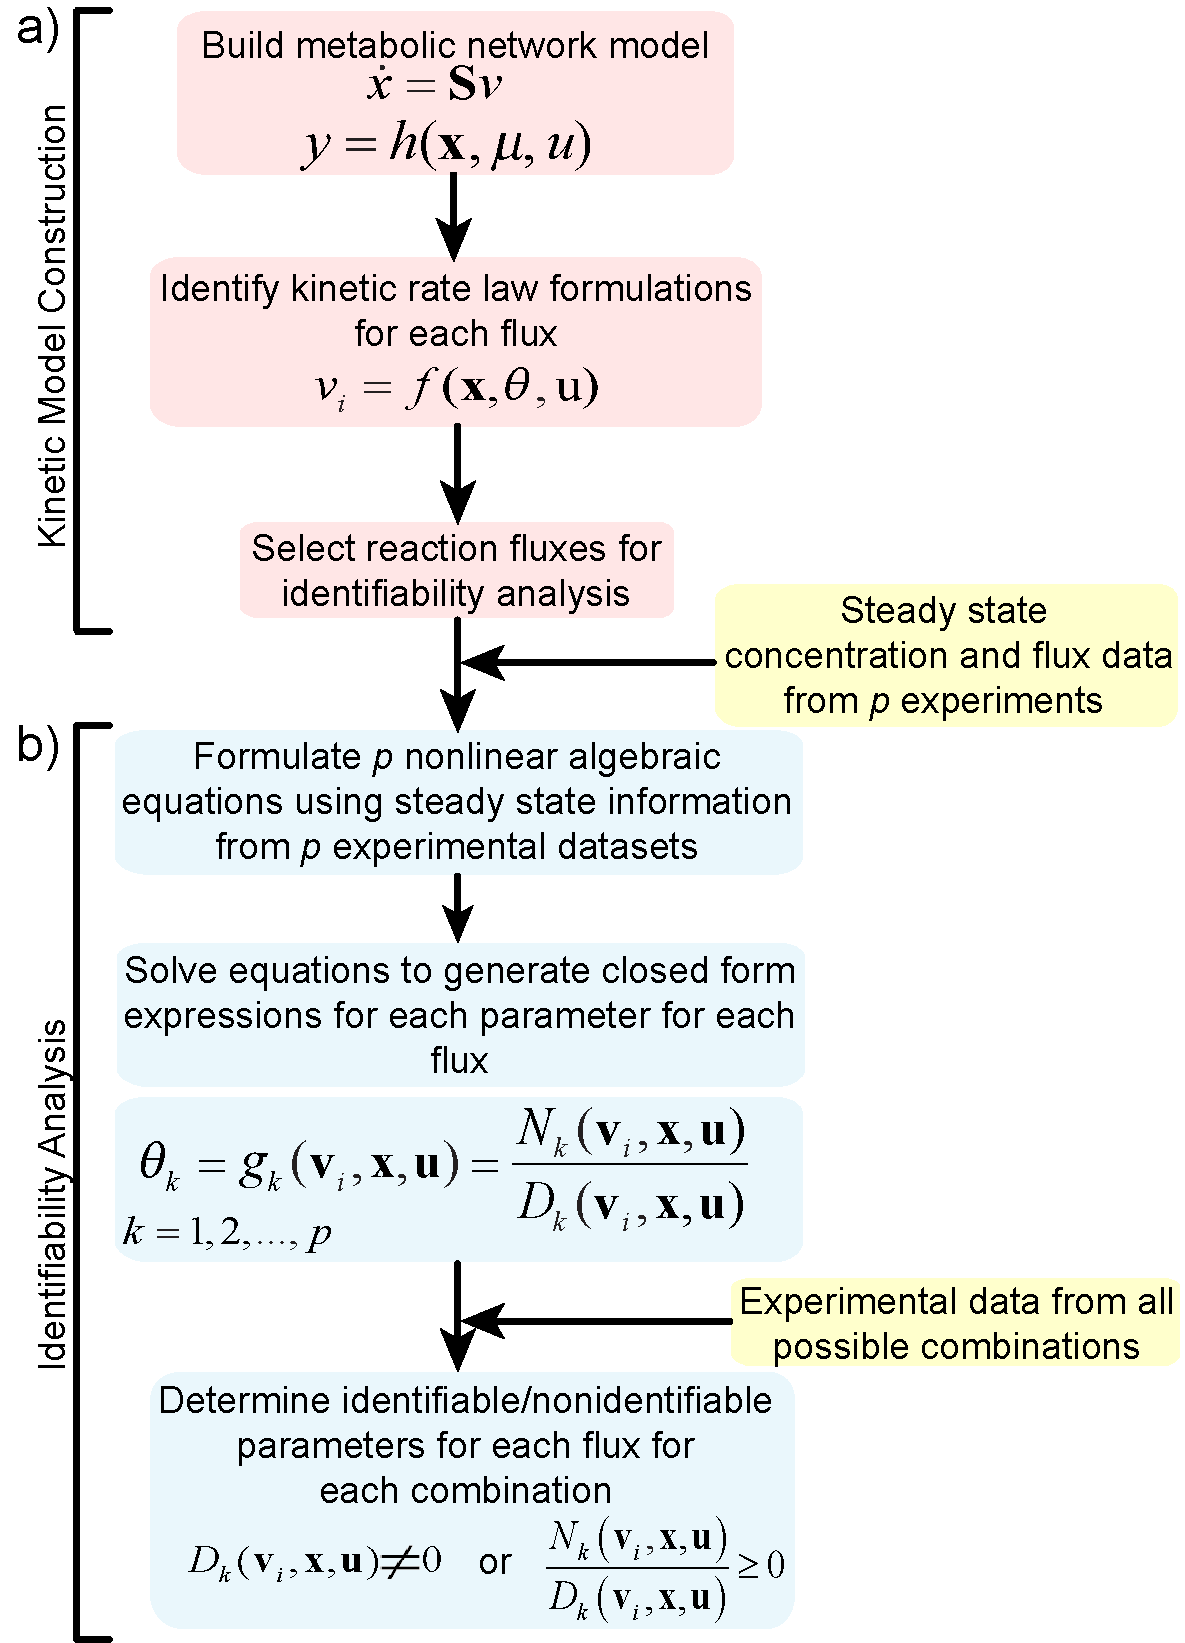
\includegraphics[width=.6\textwidth,height=.6\textheight,keepaspectratio]{figures/figure3/ident_analysis}}
		\caption{A flow diagram showing the methodology developed to establish practical identifiability of parameters in kinetic models of metabolism. a) The steps for the construction of a kinetic model of a metabolic network. The choice of rate law formulations to describe metabolic fluxes influences the identification methodology. The identifiability of parameters for each flux can be established independently. b) The steps for practical identifiability analysis for parameters of a single flux.}\label{fig:ident-flowchart}
	\end{figure}

	\begin{figure}[!tbhp]
		\centering{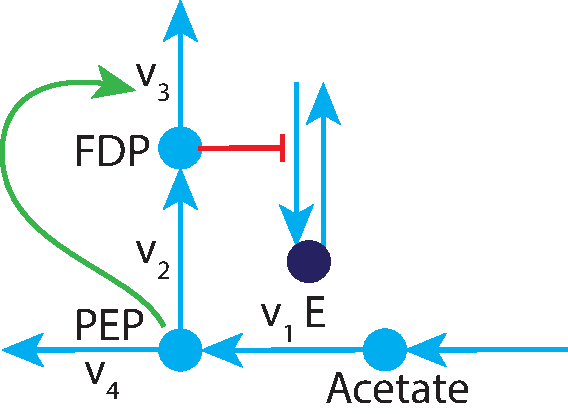
\includegraphics[width=.3\textwidth,height=.6\textheight,keepaspectratio]{figures/figure5/Figure1_NetworkA}}
		\caption{The small metabolic network for gluconeogenesis used to demonstrate our practical identifiability method for kinetic models of metabolism.}\label{fig:network}
	\end{figure}		
	
	\begin{figure}[!tbhp]
		\centering{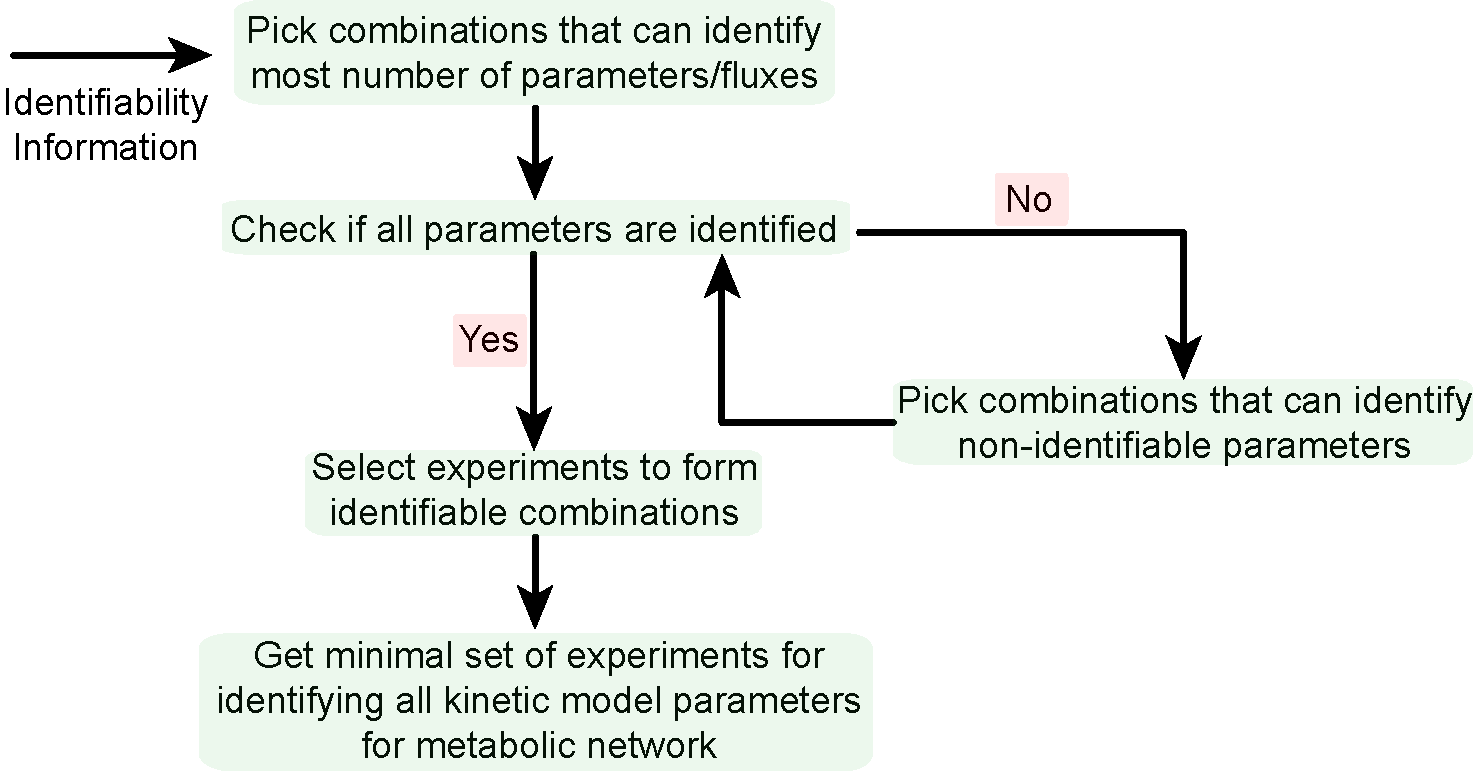
\includegraphics[width=.6\textwidth,height=.6\textheight,keepaspectratio]{figures/figure3/experimental_design}}
		\caption{Flow diagram showing a method for experimental design that uses our methodology for practical identification of parameters to determine the number and type of experiments required to identify all fluxes within a given metabolic network.}\label{fig:ident-design}
	\end{figure}

	\begin{figure}[!tbhp]
		\centering{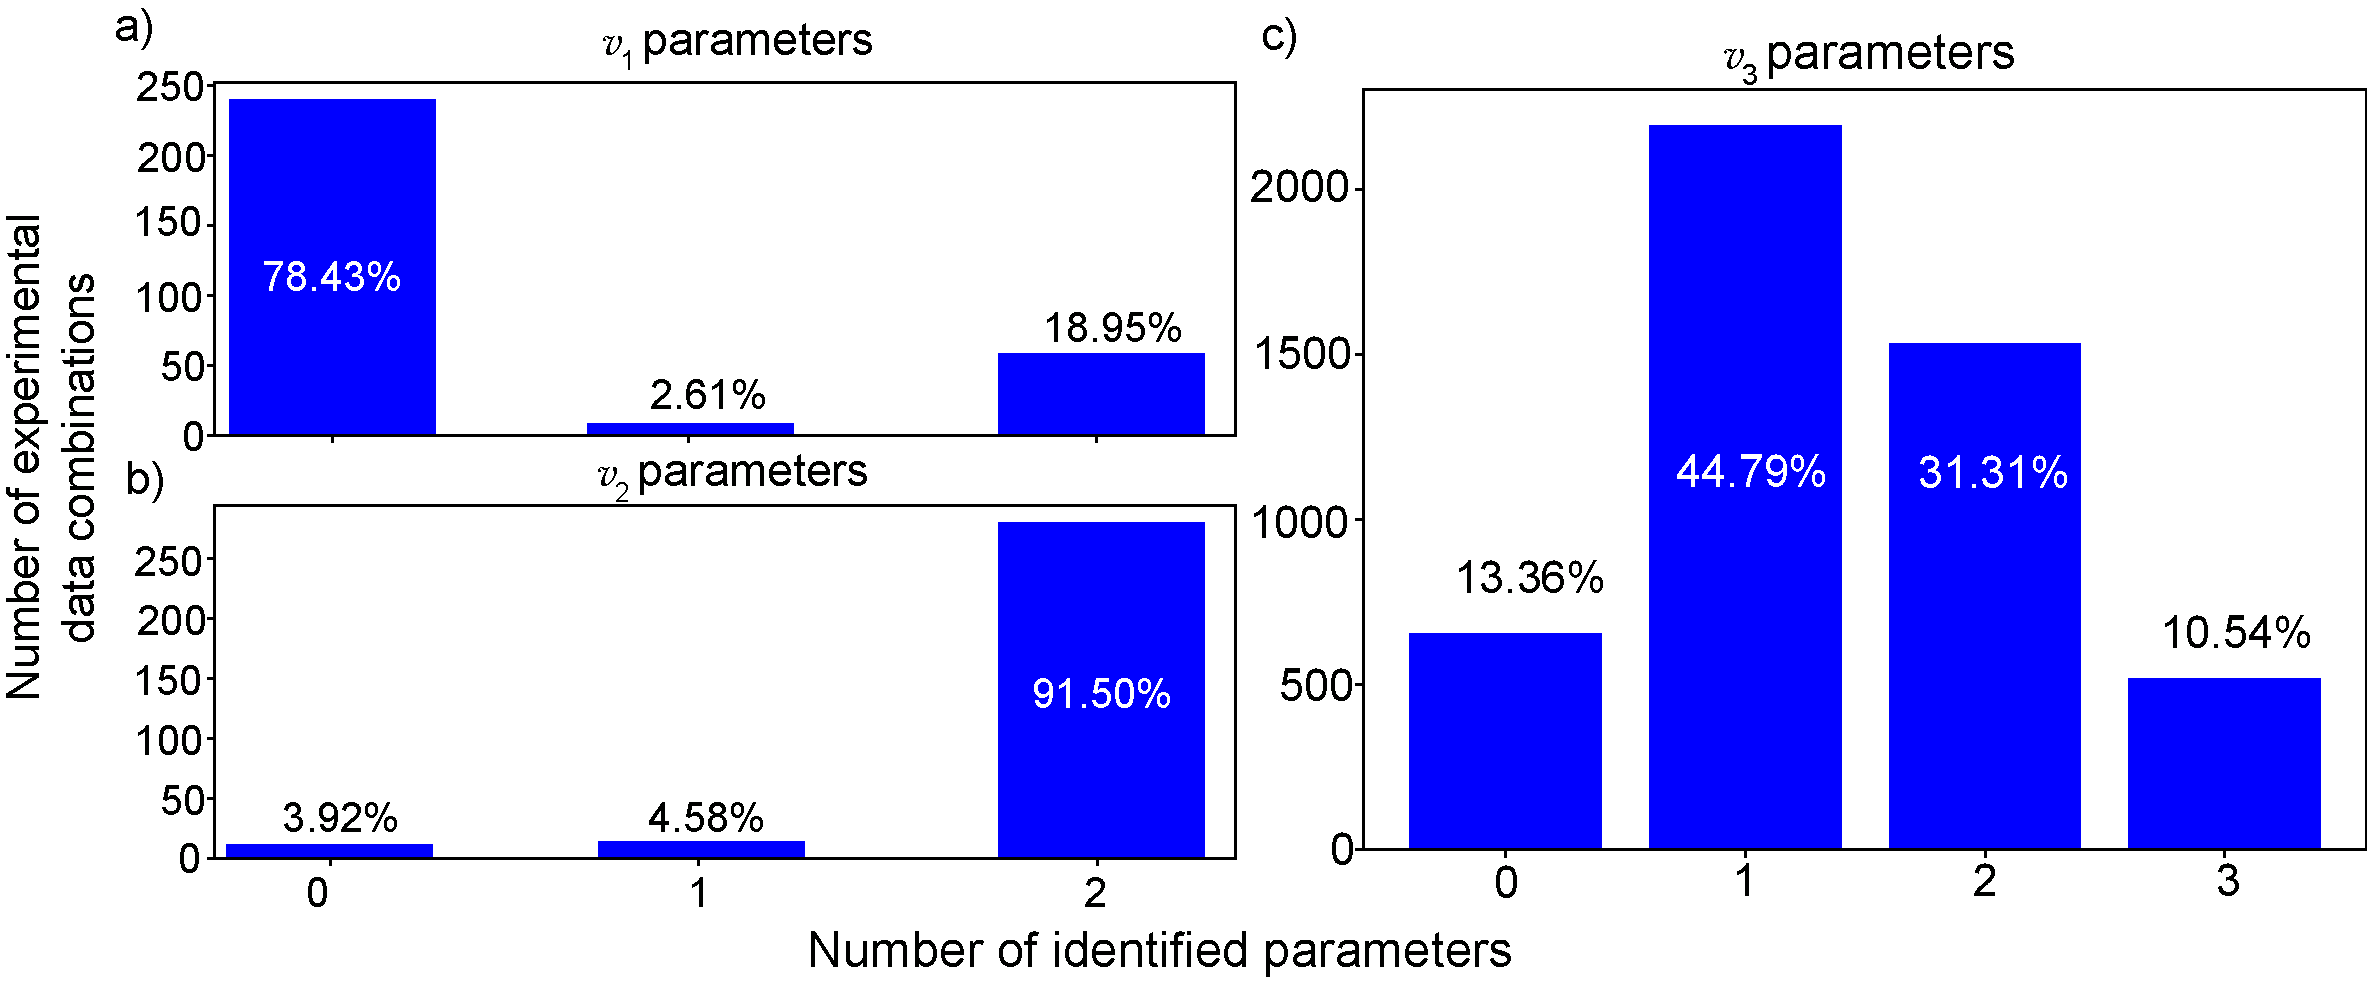
\includegraphics[width=1.0\textwidth,height=0.3\textheight]{figures/figure4/v1_V1max_v2_v3_value1_data_utility}}
		\caption{Utility of experimental data combinations on the basis of their ability to identify the most number of parameters. Information is shown for parameters modeling fluxes a) $v_1$, b) $v_2$ and c) $v_3$. The total possible number of parameters that can be identified by data from combinations of a) two, b) two, and c) three experiments is shown on the horizontal axis. The vertical axis represents the total number of combinations that can identify the corresponding number of parameters. The percentages shown in the plots represent the fraction of the total combinations used to test identifiability of parameters for a given flux. A total of 306 data combinations are used for identifiability analysis for a) $v_1$ and b) $v_2$, and 4896 combinations are used to practical identifiability of c) $v_3$. Section \ref{sec:experiments} provides more details on how the combinations of experimental data are generated.}\label{fig:figure4}
	\end{figure}	

	\begin{figure}[!tbhp]
		\centering{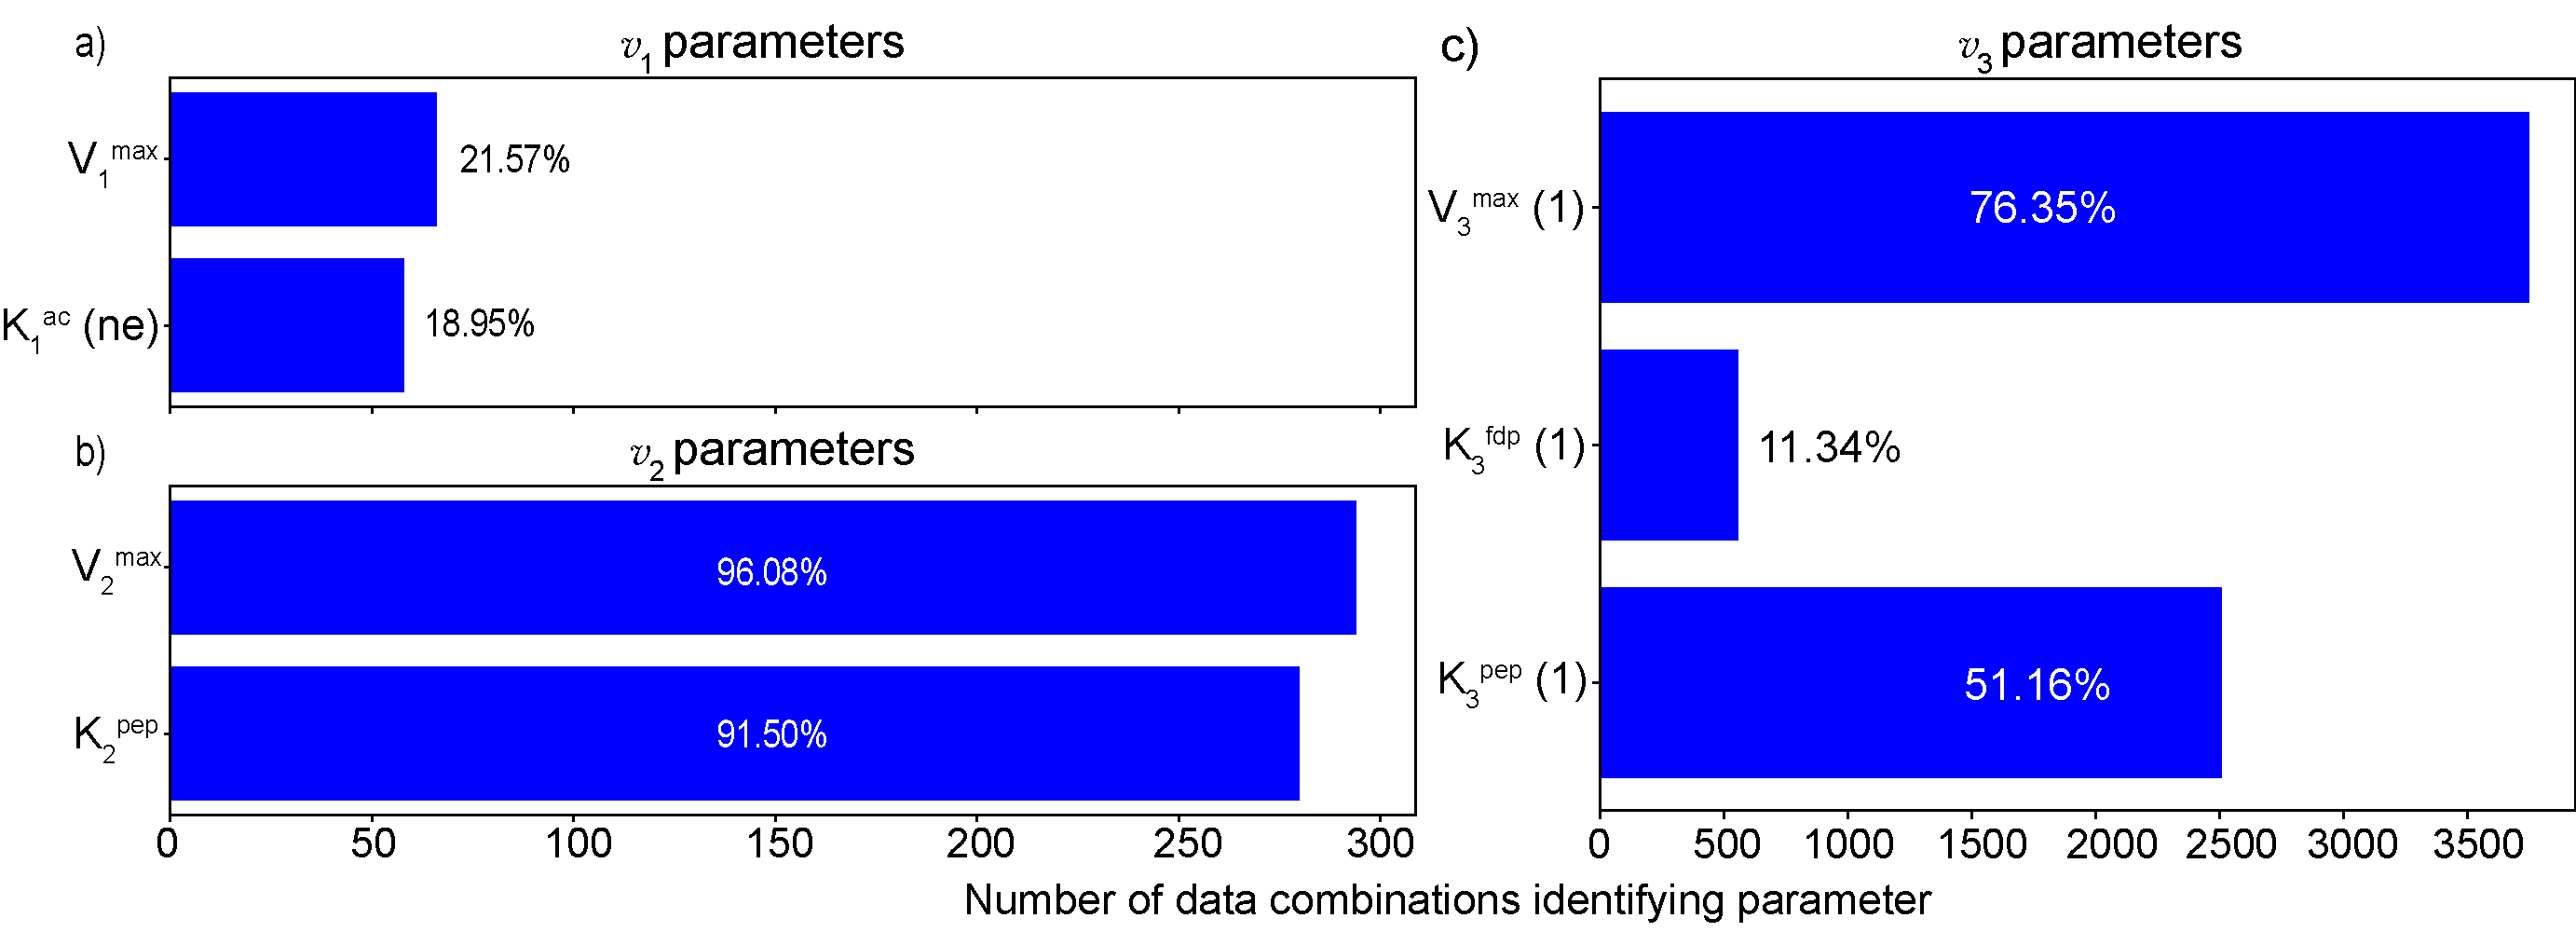
\includegraphics[width=1.0\textwidth,height=0.3\textheight]{figures/figure1/v1_V1max_v2_v3_identifiability}}
		\caption{The number of data combination from 18 different in silico experiments that can practically identify each parameter in fluxes a) $v_1$, b) $v_2$ and c) $v_3$ when there is no noise in the input experimental data. The percentage of total experimental data combinations that can identify each parameter is specified either in, or right next to the bar showing the total number of combinations identifying a given parameter. Since the total number of experiments used to identify parameters in $v_1$ and $v_2$ is two, the total number of data combinations used to identify parameters in fluxes $v_1$ and $v_2$ is lower (at 306) that the total number of combinations used to test identifiability of parameters for $v_3$ (at 4896), which is modeled with three parameters and requires data from at least three different experiments.}\label{fig:figure1}
	\end{figure}

	\begin{figure}[!tbhp]
		\centering{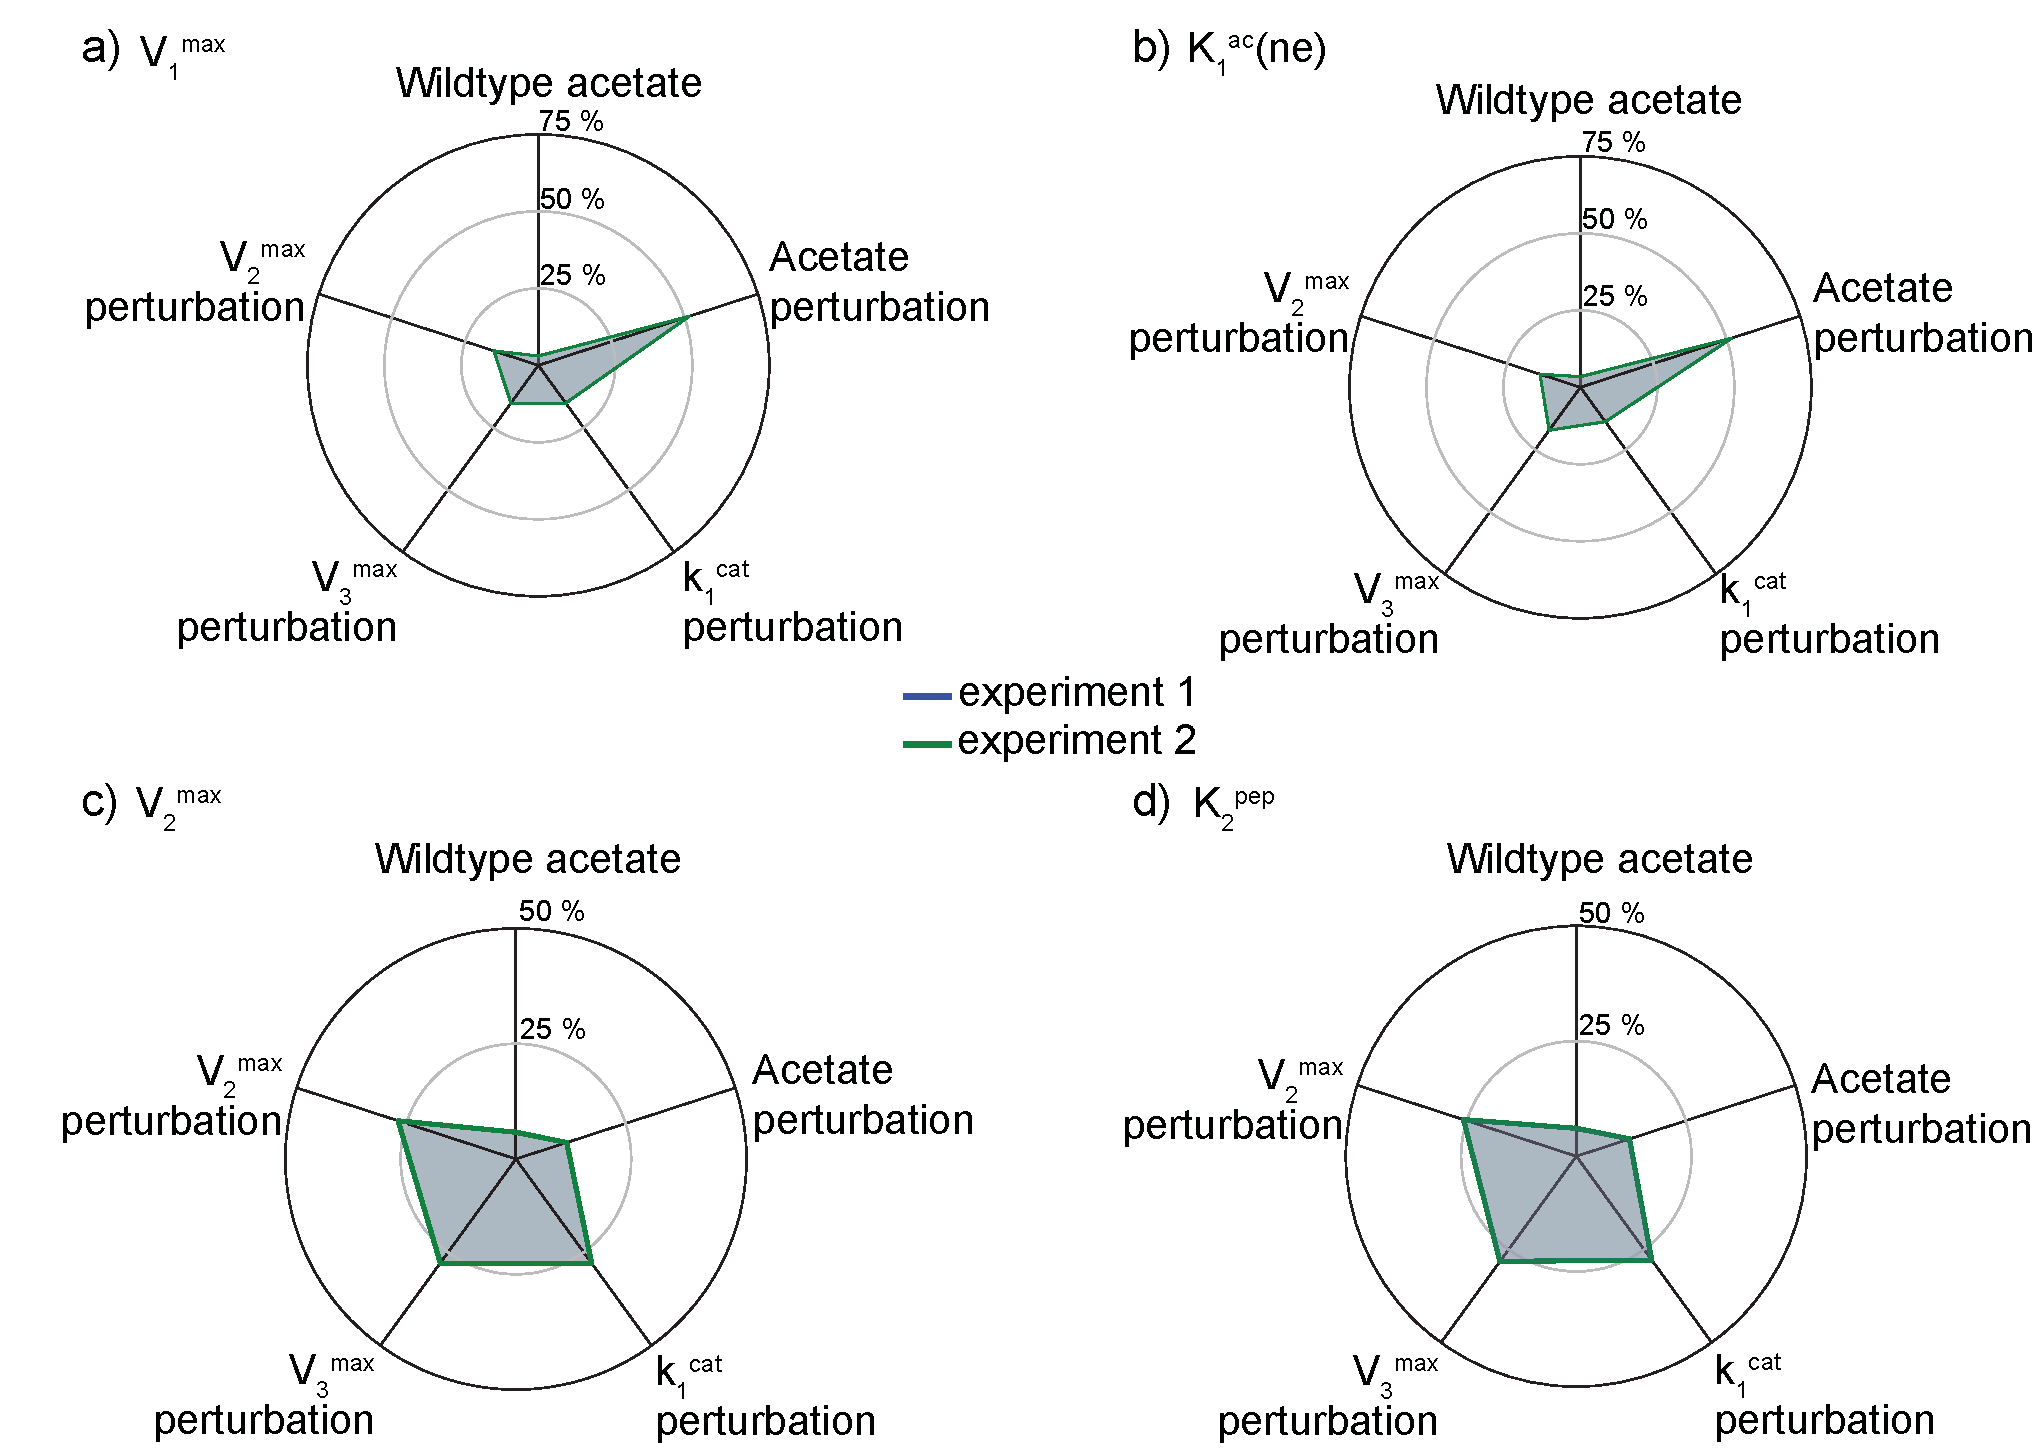
\includegraphics[width=1.0\textwidth,height=0.6\textheight, keepaspectratio]{figures/figure2/v1_V1max_only_v2_spider}}
		\caption{The contribution of different experiments types used in a combination of two experiments ($k = \{1, 2\}$) that can practically identify parameter a) $V_1^{max}$, b) $K_1^{ac}$, c) $V_2^{max}$ and d) $K_2^{pep}$. The percentages reflect the fractional contribution of each experiment type towards all identifiable data combinations.}\label{fig:figure2}
	\end{figure} 
	
\end{document}